\documentclass[hyperref,UTF8,12pt,a4paper]{ctexart}
\usepackage{amsmath}
\usepackage{amsfonts}

\usepackage{geometry}
\usepackage{tikz}
\geometry{left=1in,right=1in,top=1in,bottom=1in}

\hypersetup{
	colorlinks=true,
	linkcolor=black
}
\ctexset{abstractname=\zihao{2}摘\quad{}要}

\usepackage{titling}
\pretitle{\begin{center}\fontsize{30pt}{30pt}\selectfont}
\posttitle{\end{center}}

\usepackage{fancyhdr}
\pagestyle{fancy}
\fancyhf{}
\fancyhfoffset[L]{0cm} % left extra length
\fancyhfoffset[R]{0cm} % right extra length
\chead{网络空间安全导论报告}
\rfoot{}

\usepackage{ulem}

\title{浅谈 ReDoS 的攻击与防御}
\author{罗江楠}
\date{2021.10.23}

\begin{document}
\maketitle

\newpage

\tableofcontents

\newpage

\begin{abstract}

\vspace{\baselineskip}

正则表达式拒绝服务攻击(ReDoS)漏洞是一种常见且严重的算法复杂度攻击漏洞,并在近年呈增长趋势。
本文从目前常用的正则表达式引擎和算法角度,阐述了基于 NFA-$\varepsilon$ 算法的主流正则表达式匹配算法,
并且分析了其拥有的致命缺陷,以及会导致缺陷呈指数级放大的 ReDoS 攻击原理。
在文章的最后,本文介绍了一些常用的防御 ReDoS 的手段,以及一些在关于自动检测 ReDoS 风险方面的最新进展。

\par\textbf{关键词:}正则表达式; ReDoS; NFA;

\end{abstract}

\newpage

\section{ReDoS 简介}

Web 攻击是一个非常常见和热门的课题,攻击的手段也多种多样,常见的攻击方式不外于一下几个大方面:

\begin{itemize}
\item SQL 注入攻击
\item XSS 跨站脚本攻击
\item CSRF 跨站请求伪造攻击
\item 文件上传漏洞攻击
\item DDoS 分布式拒绝服务攻击
\item 其他攻击
\end{itemize}

本文将要介绍的正则表达式拒绝服务攻击(ReDoS)是属于拒绝服务攻击(DoS)中的一个子类,但是却与分布式拒绝服务攻击(DDoS)不同。ReDoS 利用的是一般程序语言在正则表达式匹配算法的实现方面的缺陷,使得目标服务器在短期内消耗大量资源,从而实现拒绝服务攻击。

然而 ReDoS 并不是通用的,该漏洞只在一些有缺陷的正则表达式中才能触发。反之,想要防范 ReDoS 攻击,也只需要排查自身源代码中是否有含有缺陷的表达式即可。

\section{正则表达式回退式匹配算法}

在大部分计算机语言的标准库中,用于匹配正则表达式的算法是基于 NFA-$\varepsilon$ 的通用算法。

NFA 全称为非确定有限状态自动机,是对每个状态和输入符号对可以有多个可能的下一个状态的有限状态自动机。
与其相反的则是确定有限状态自动机(DFA),它的下一个可能状态是唯一确定的。

尽管 NFA 和 DFA 在定义上不同,但是在形式理论中可以证明它们是等价的。
通过使用幂集构造,我们可以将两者轻松转化。
而 NFA-$\varepsilon$ 则是有 $\varepsilon$ 移动的 NFA,它允许到新状态的变换不消耗任何输入符号。
% 常见的正则表达式引擎使用的都是基于 NFA-$\varepsilon$ 的正则表达式匹配算法,
% 而 NFA-$\varepsilon$ 算法最致命的缺陷便是在通过幂集构造转化为 DFA 时最劣复杂度能达到 $O(2^n)$ 级别。

\subsection{NFA-$\varepsilon$ 的建图算法}

NFA-$\varepsilon$ 的本质是一张有向图,其中包括一个起始点 $S$ 和终止点 $T$。
其中待匹配的字符串从 $S$ 出发,每经过一条边,就从字符串的头部删去一个相应的字符。
特别的,如果经过的是一条 $\varepsilon$ 边,则不需要删去任何字符就可以到达下一个节点。
如果字符串能够刚好在到达 $T$ 的时候用完全部的字符,则我们可以得出字符串与正则表达式匹配的结论。

从只包含一个字符的正则表达式看起,我们只需要将 $S$ 直接连一条匹配字符的边到 $T$ 即可,如图 1。

\begin{figure}[h]
	\centering
	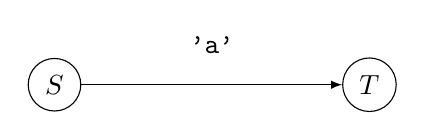
\begin{tikzpicture}
		\node[circle,draw=black] (1) at(0,0) {$S$};
		\node[circle,draw=black] (2) at(4,0) {$T$};
		\draw[-latex] (1)--(2);
		\node at(2,0.5) {\verb|'a'|};
	\end{tikzpicture}
	\caption{匹配单个字符的 NFA}
\end{figure}

对于 \verb!<regex> <regex>! 的顺序连接形式,我们只需要将第一个 NFA 的 $T$ 点连一条 $\varepsilon$ 边到第二个 NFA 的 $S$ 点即可。新的 NFA 的 $S$ 点即为 $S_1$,$T$ 点即为 $T_2$,如图 2。

\begin{figure}[h]
	\centering
	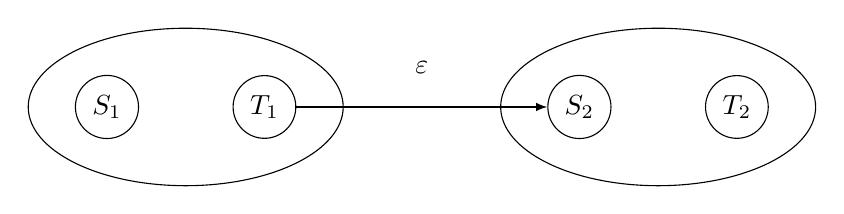
\begin{tikzpicture}
		\node[circle,draw=black] (1) at(2,0)  {$S_1$};
		\node[circle,draw=black] (2) at(4,0)  {$T_1$};
		\node[circle,draw=black] (3) at(8,0)  {$S_2$};
		\node[circle,draw=black] (4) at(10,0) {$T_2$};
		\draw[-latex] (2)--(3);
		\node at(6,0.5) {$\varepsilon$};
		\draw (3,0) ellipse (2 and 1);
		\draw (9,0) ellipse (2 and 1);
	\end{tikzpicture}
	\caption{顺序连接两个表达式的 NFA}
\end{figure}

对于 \verb!<regex> | <regex>! 或者 \verb|[<atom-regex-list>]| 的逻辑或形式,我们需要新建两个节点 $S$ 和 $T$,然后从 $S$ 节点向各个 $S_i$ 节点连 $\varepsilon$ 边,从各个 $T_i$ 节点向 $T$ 节点连 $\varepsilon$ 边。$S$ 和 $T$ 即为新 NFA 的起始点和终止点,如图 3。

\begin{figure}[h]
	\centering
	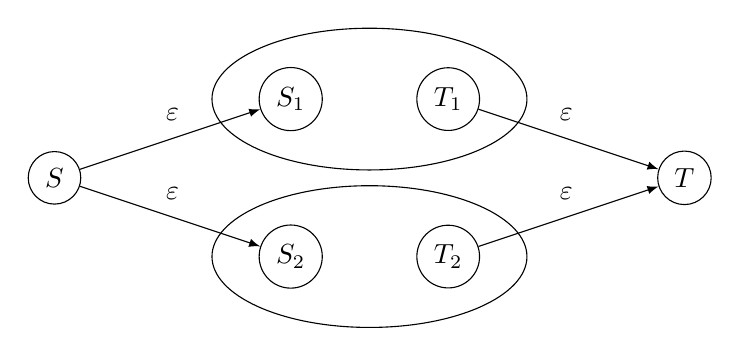
\begin{tikzpicture}
		\node[circle,draw=black] (1) at(2,0) {$S_2$};
		\node[circle,draw=black] (2) at(4,0) {$T_2$};
		\node[circle,draw=black] (3) at(2,2) {$S_1$};
		\node[circle,draw=black] (4) at(4,2) {$T_1$};
		\node[circle,draw=black] (5) at(-1,1) {$S$};
		\node[circle,draw=black] (6) at(7,1) {$T$};
		\draw[-latex] (5)--(1);
		\draw[-latex] (5)--(3);
		\draw[-latex] (2)--(6);
		\draw[-latex] (4)--(6);
		\draw (3,0) ellipse (2 and 0.9);
		\draw (3,2) ellipse (2 and 0.9);
		\node at(0.5,0.8) {$\varepsilon$};
		\node at(0.5,1.8) {$\varepsilon$};
		\node at(5.5,0.8) {$\varepsilon$};
		\node at(5.5,1.8) {$\varepsilon$};
	\end{tikzpicture}
	\caption{匹配分支形式的 NFA}
\end{figure}

对于出现一次或者多次的逻辑,即 \verb|<regex> +| 语法,我们可以直接连一条 $T$ 到 $S$ 的 $\varepsilon$ 边,如图 4。

\begin{figure}[h]
	\centering
	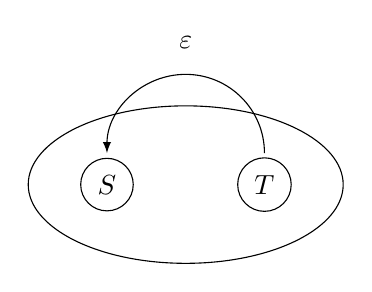
\begin{tikzpicture}
		\node[circle,draw=black] (1) at(2,0) {$S$};
		\node[circle,draw=black] (2) at(4,0) {$T$};
		\draw (3,0) ellipse (2 and 1);
		\draw[-latex] (4,0.4) arc (0:180:1);
		\node at(3,1.8) {$\varepsilon$};
	\end{tikzpicture}
	\caption{匹配一次或多次的 NFA}
\end{figure}

对于出现零次或一次的逻辑,即 \verb|<regex> ?| 语法,我们可以通过类似分支形式的方式实现,如图 5。

\begin{figure}[h]
	\centering
	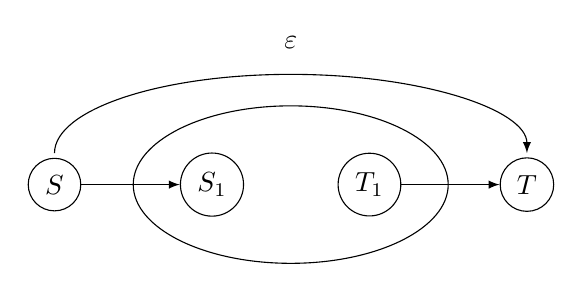
\begin{tikzpicture}
		\node[circle,draw=black] (1) at(2,0) {$S_1$};
		\node[circle,draw=black] (2) at(4,0) {$T_1$};
		\node[circle,draw=black] (3) at(0,0) {$S$};
		\node[circle,draw=black] (4) at(6,0) {$T$};
		\draw (3,0) ellipse (2 and 1);
		\draw[-latex] (3)--(1);
		\draw[-latex] (2)--(4);
		\draw[-latex] (0,0.4) arc (180:0:3 and 1);
		\node at(3,1.8) {$\varepsilon$};
	\end{tikzpicture}
	\caption{匹配零次或一次的 NFA}
\end{figure}

对于最后一种出现零次、一次或多次的逻辑,即 \verb|<regex> *| 语法,我们可以将其拆解为 \verb|(<regex> +) ?| 的形式,建图的方法是上述两种方法的叠加,本文不再进行赘述。

综上所述,我们可以按照上面的方案对于每个给定的正则表达式都建出一个相应的 NFA-$\varepsilon$,并且通过这个 NFA-$\varepsilon$ 来完成正则表达式匹配的计算。

\subsection{NFA-$\varepsilon$ 的匹配算法}

想要在 NFA-$\varepsilon$ 上进行字符串的匹配,则需要用类似深度优先搜索的办法,
在每次转移到下一个状态节点的时候同时记录状态的节点和字符串中当前匹配的位置。
当在某个节点失配的时候(或者是没有其他可以继续前进的状态节点时),回退到先前的状态,
并且重新选择不同的分支继续进行匹配的尝试。

让我们分析一个最简单的可用于 ReDoS 攻击的一个具有缺陷的正则表达式:

$R=$ \verb|^(a+)+$|

这个表达式构造出来的 NFA-$\varepsilon$ 如图 6。

\begin{figure}[h]
	\centering
	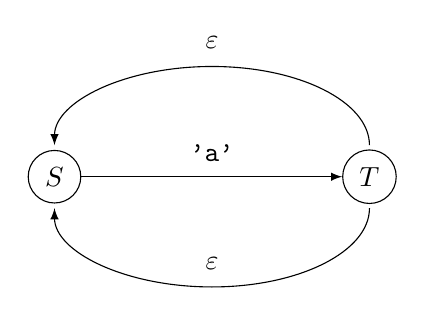
\begin{tikzpicture}
		\node[circle,draw=black] (1) at(0,0) {$S$};
		\node[circle,draw=black] (2) at(4,0) {$T$};
		\draw[-latex] (1) --(2);
		\draw[-latex] (4,0.4) arc (0:180:2 and 1);
		\draw[-latex] (4,-0.4) arc (0:-180:2 and 1);
		\node at(2,1.7) {$\varepsilon$};
		\node at(2,-1.1) {$\varepsilon$};
		\node at(2,0.3) {\verb|'a'|};
	\end{tikzpicture}
	\caption{带有缺陷的 NFA}
\end{figure}

可以看到,套有双层加号的正则表达式在 NFA-$\varepsilon$ 上会出现两条相同的 $\varepsilon$ 边从 $T$ 连向 $S$,
而这两条相同的 $\varepsilon$ 边正是导致 NFA-$\varepsilon$ 匹配算法复杂度暴增的主要原因。
我们可以用一个具体的样例来说明问题的存在,让我们尝试匹配一下这个字符串:$s=$ \verb|"aaaaaaaaaaX"|。
非常显然,字符串 $s$ 并不能匹配正则表达式,然而让我们来模拟一下判断匹配的算法需要计算多少步才能得出结论。

最开始我们位于点 $S$,并且字符串 $s$ 的已匹配长度为 $0$,我们就将这个状态记为 $\{S, 0\}$。
之后我们尝试寻找从 $S$ 的出边,我们能够找到一条连往 $T$ 并且匹配字符 \verb|'a'| 的边,
于是我们前进到 $T$ 点,并且当前状态变成 $\{T, 1\}$。
接下来寻找到两条从 $T$ 的出边,并且都是 $\varepsilon$ 边,于是我们随便找一条边,并且前进到下一个状态 $\{S, 1\}$。

这是我们第一次回到 $S$ 点,接下来我们就会重复上面的步骤,直到我们第十次回到 $S$ 点时,当前状态是 $\{S, 10\}$,
并且下一个字符 \verb|'X'| 无法再找到能够匹配的边继续前进,于是我们便开始回退。当回退到上一步 $\{T, 10\}$ 时,
我们会选择另外一条 $\varepsilon$ 边,并且重新前进到 $\{S, 10\}$ 再次尝试匹配。

让我们分析一下这个过程的复杂度。让我们设 $T(n)$ 表示当我们搜索到 $\{S, n\}$ 时的复杂度。
当 $n < 10$ 时,非常容易得知,通过 $\{S, n\}$ 的状态我们可以直接转移到 $\{T, n\}$ 的状态,
之后再可以通过两条 $\varepsilon$ 边转移到 $\{S, n+1\}$ 的状态。也就是说我们有以下的转移方式:

\[
	T(n) = 2 T(n+1) (n < 10)
\]

而当 $n = 10$ 时,状态 $\{S, 10\}$ 无法转移至任何其他的状态,因此我们可以得到递归的结束状态 $T(10) = 1$。

因此,我们可以通过计算,得知 $T(1) = 2^9 = 2^{n-1}$。
也就是说,对于一个开头长度为 $n$ 的 \verb|'a'| 重复加上最后一个其他字符的字符串,
能够将基于回退算法的正则表达式匹配算法卡至理论最差复杂度 $O(2^n)$。

因此如果我们仅仅只将开头字符 \verb|'a'| 的数量增长到 $100$ 的级别,
那么一般的计算机便无法在短暂的时间内完成正则表达式的匹配计算,
并且逐渐将服务器的资源耗尽,最终使得服务器无法正常对外提供服务。

\section{其他正则表达式匹配算法}

基于回退式的正则表达式匹配算法虽然具有缺陷,但却是非常普遍运用在各种编程语言的正则标准库中。

正则表达式引擎主要可以实现为 DFA 或者 NFA。更加一般来讲,我们可以将正则表达式引擎可以大致分为两类。

\begin{itemize}
	\item 文本导向:引擎在从一个字符移动到下一个字符之前会尝试正则表达式中的所有的可能路径。也就是说,引擎会保存当前字符在自动机上所有可以到达的点,并且在下一次的移动中会对于所有的点尝试进行移动,最后返回整个字符串最远能够到达的点。该算法不会回溯,但是同样的会消耗许多的内存空间。
	\item 正则表达式导向:使用类似深度优先搜索算法的顺序进行搜索,每当一个位置无法再进行匹配的时候就会回溯到上一状态,并且从其他路径重新进行匹配搜索。一般来讲,搜索的顺序是从不同分支从左到右进行的,因此基于该算法的匹配算法将会返回可能的最左边的匹配结果。
\end{itemize}

由于在实际的应用情况中,若要实现正则表达式中例如惰性量词、反向引用等特性,使用第二种正则表达式导向的引擎是唯一的办法。
因此尽管大家都知道正则表达式导向的引擎有如此严重的漏洞,但我们只能从自身开始进行防范。

\begin{figure}[h]
	\centering
	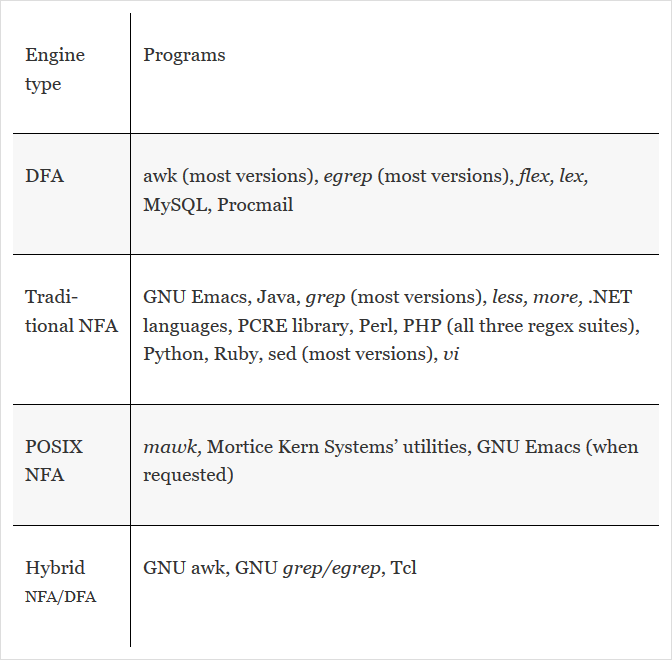
\includegraphics[width=15cm]{figures/languages.png}
	\caption{不同语言标准库中正则匹配所用的算法}
\end{figure}

\newpage

\bibliographystyle{plain}

\begin{thebibliography}{99}
\bibitem{a} 我也不知道是什么东西

\end {thebibliography}

\end{document}
